\section{Calibration Process Design}
\label{sec:desaindanimplementasi1}

Omnivision Camera Calibration using Machine Learning methods consists of two things, namely the calibration data acquisition process and the calibration data learning process. The calibration data acquisition process is worked by humans by matching data from the camera with real world data. Meanwhile, the learning process is carried out by a computer using the Multi-Layer Perceptron method which will be made into a Lookup Table.

\subsection{Data Acquisition}
\label{sec:deskripsisistem}

\begin{figure}[H]
  \centering
  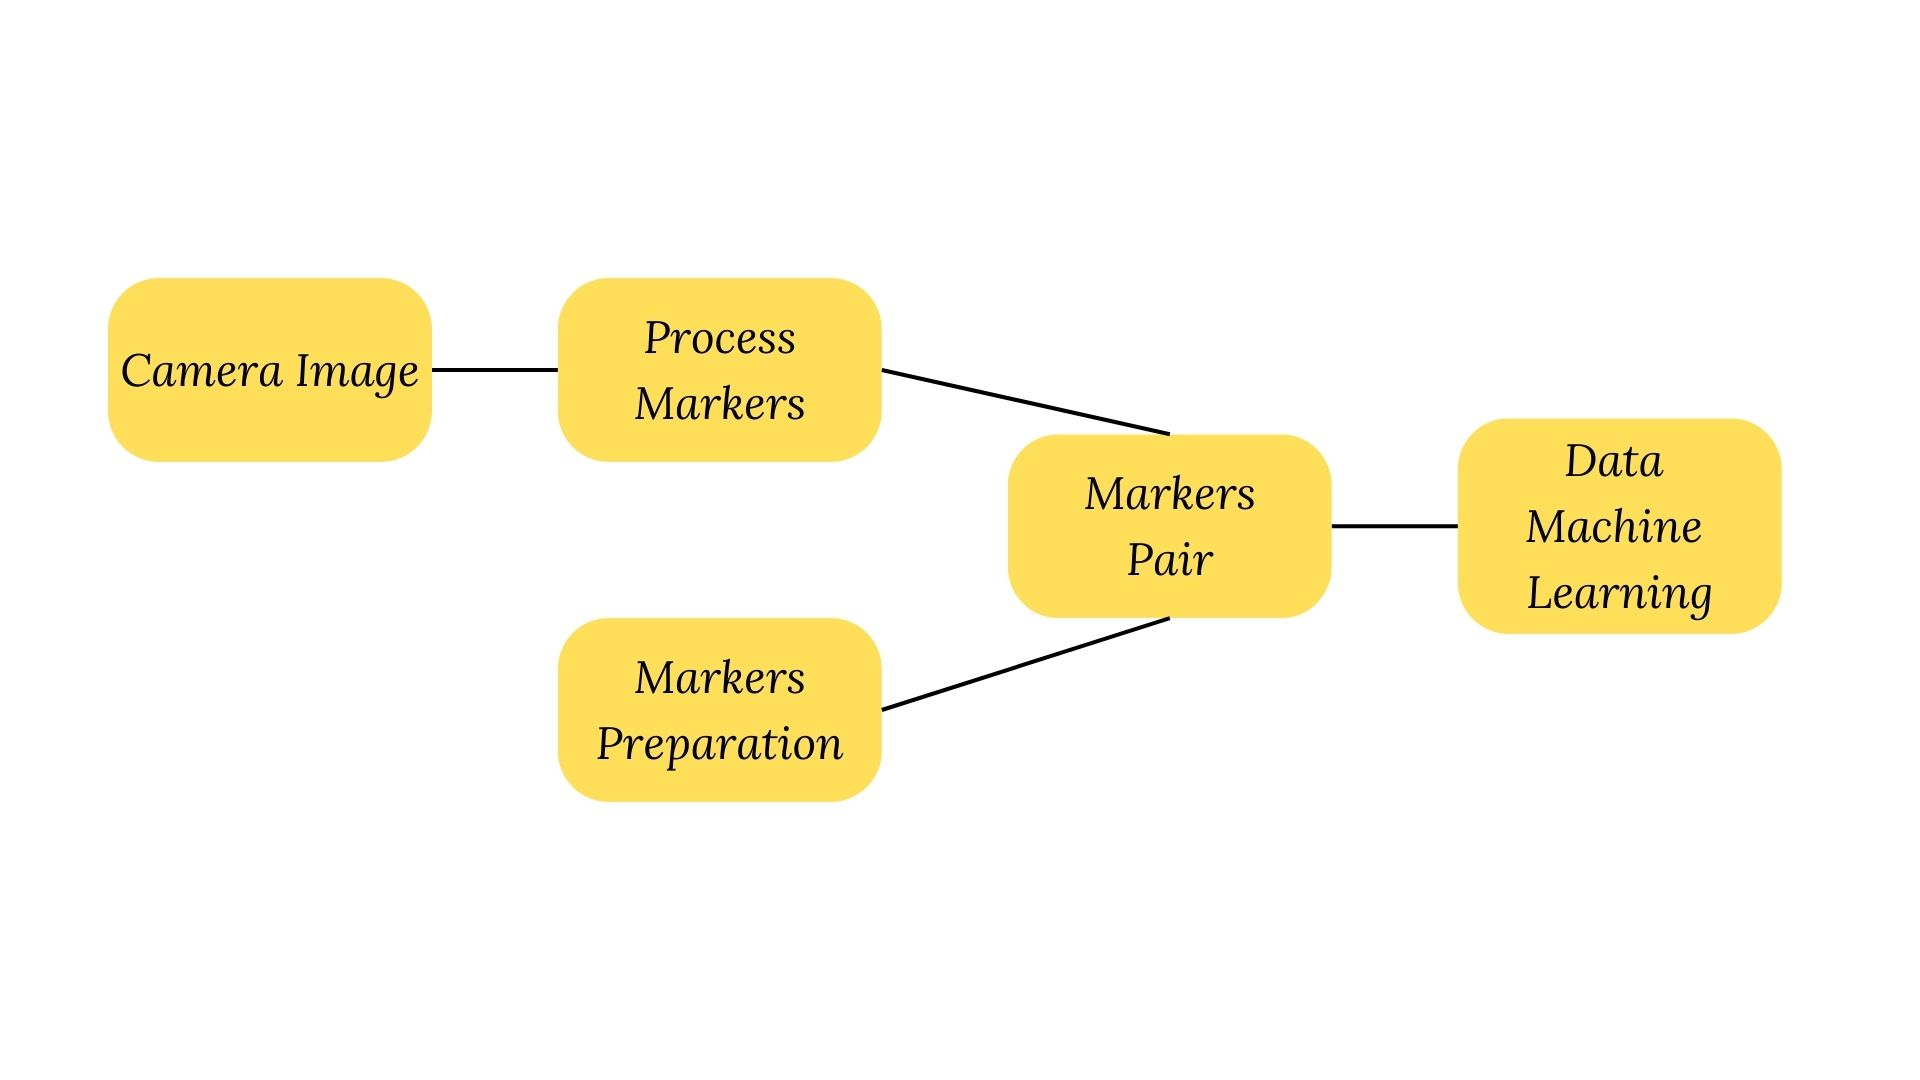
\includegraphics[width=8cm]{gambar/anu2.jpg}
  \caption{Data Acquisition Block Diagram.}
  \label{fig:diag31}
\end{figure}

The first thing to do is to get an image from the Omnivision camera. This can be obtained through a program made by the author. The program will display the camera image on the website. Here is the image of the website that displays the Omnivision camera image: 

\begin{figure}[H]
  \centering
  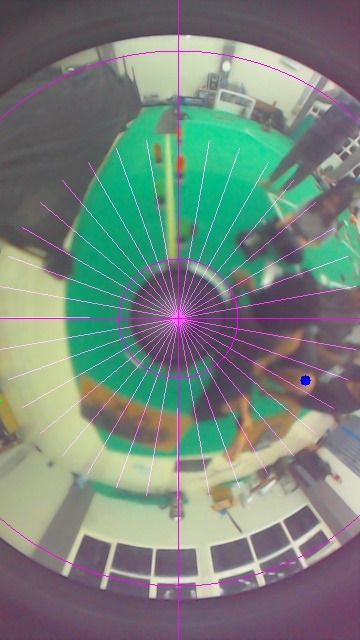
\includegraphics[width=6cm]{gambar/iris_web.jpeg}
  \caption{Camera Image View.}
  \label{fig:diag310}
\end{figure}

Next step is to prepare markers in the field. The markers are arranged according to the desired data. The placement of the markers varies from 60 cm to 460 cm from the robot. Here is the image of the marker placement in the field:

\begin{figure}[H]
  \centering
  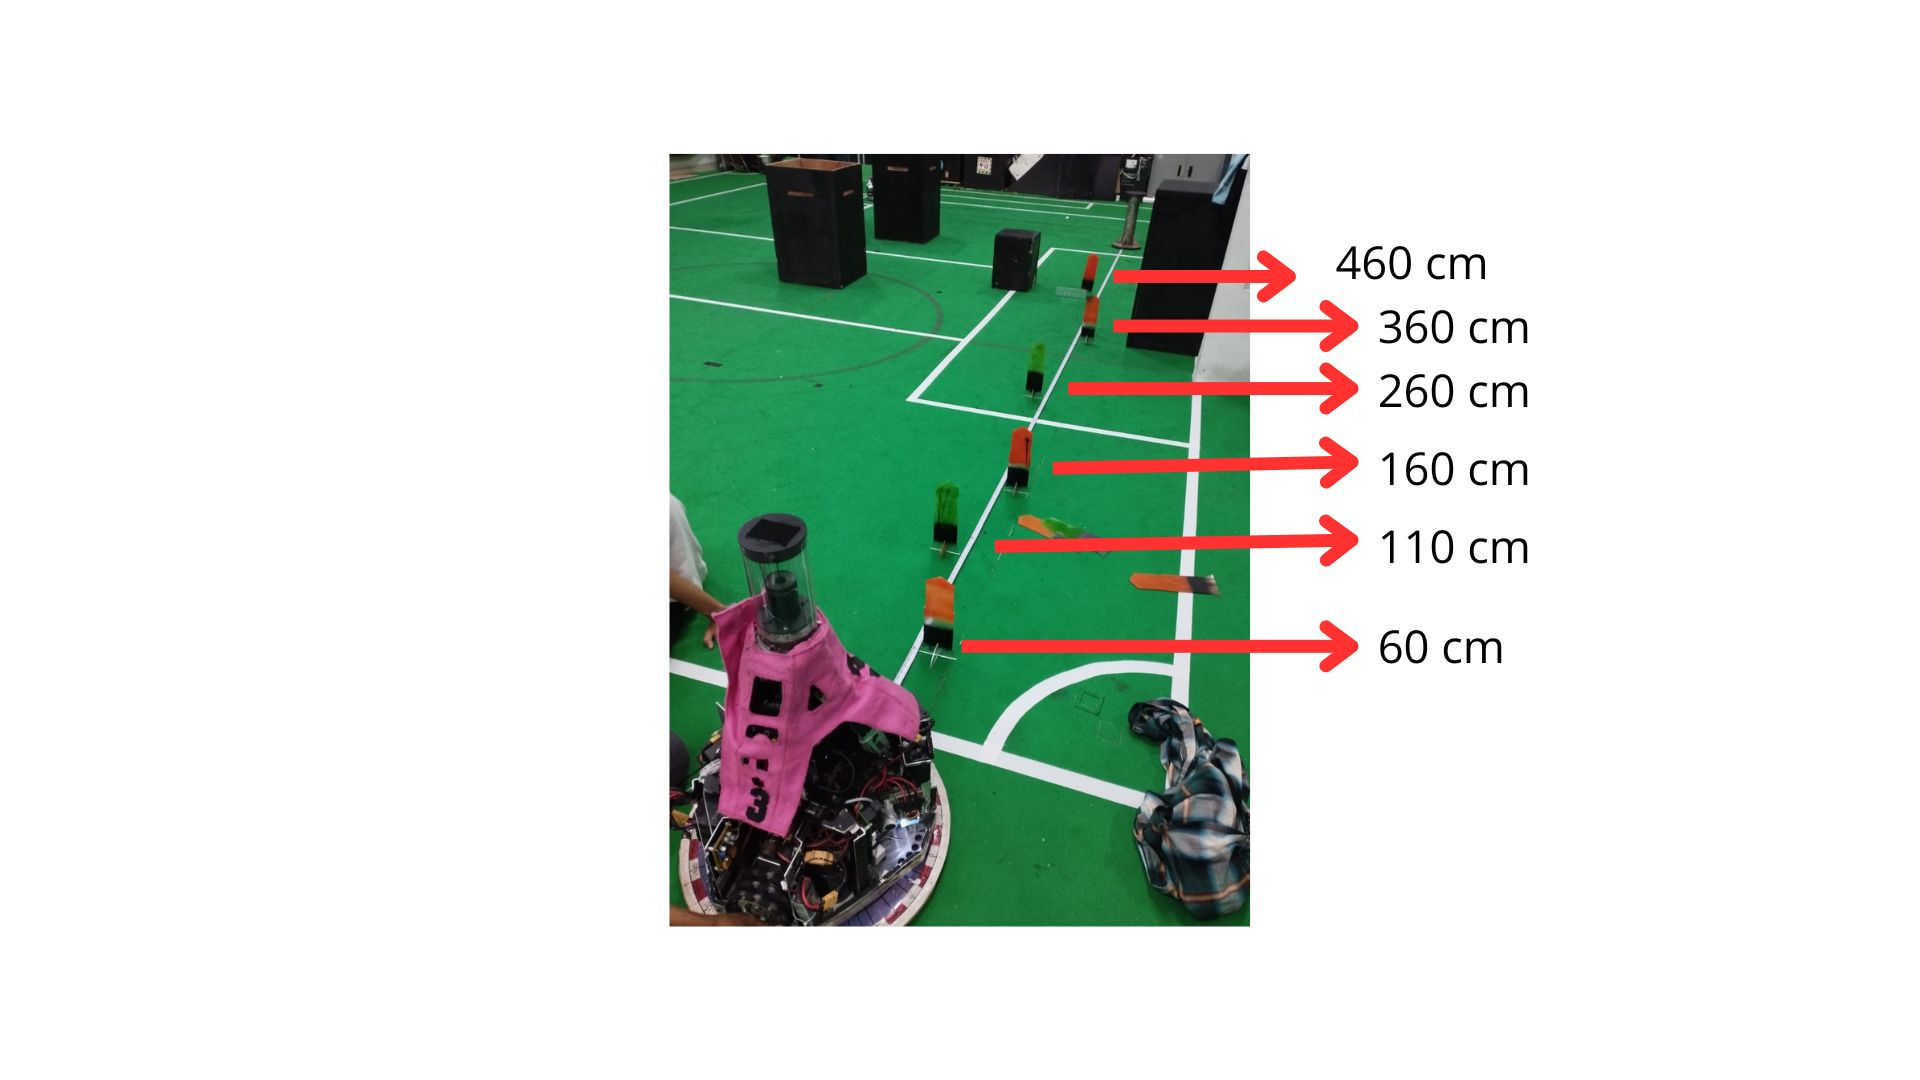
\includegraphics[width=12cm]{gambar/ambil_data_new.jpg}
  \caption{Markers on Field.}
  \label{fig:diag311}
\end{figure}

Next step is to process the markers on the camera coordinates. 

\begin{figure}[H]
  \centering
  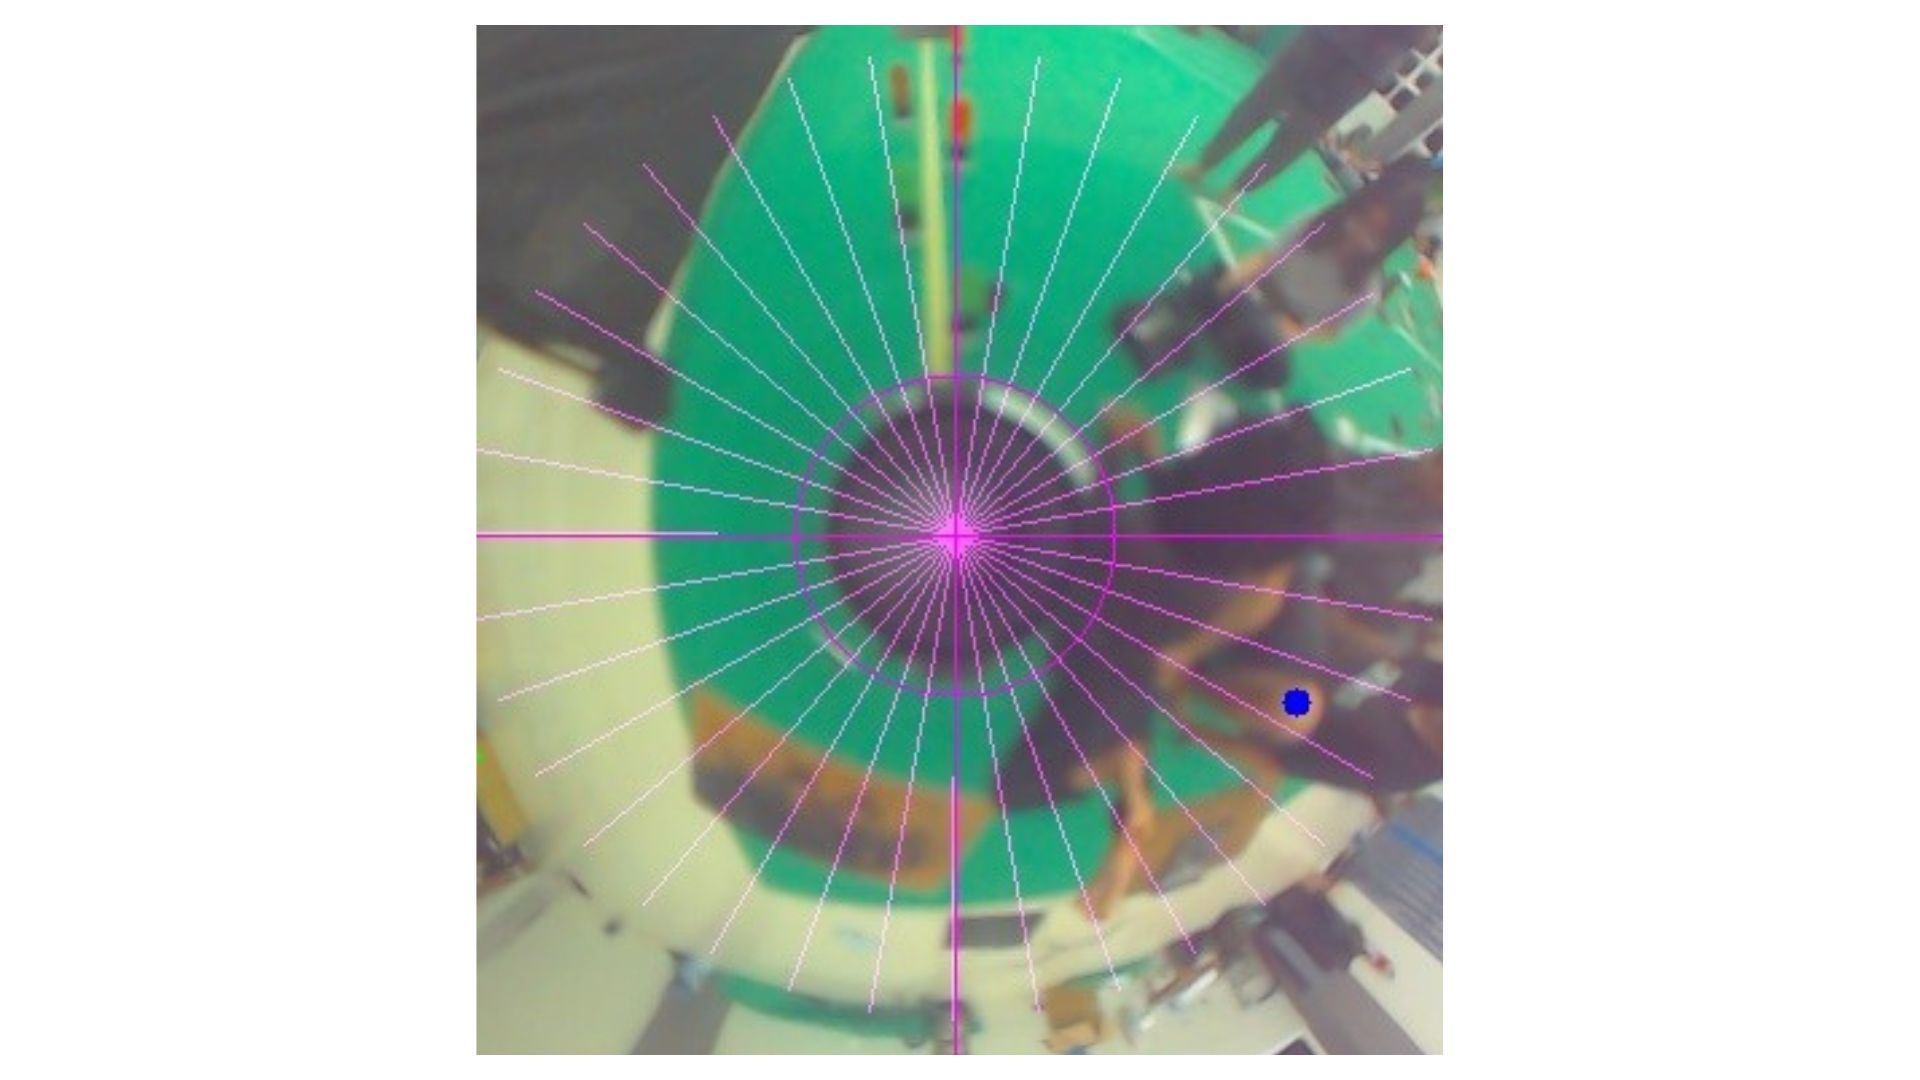
\includegraphics[width=10cm]{gambar/web_zoom.jpg}
  \caption{Camera Image View Zoomed.}
  \label{fig:diag312}
\end{figure}

From that website, the markers on the image can be clicked to get the coordinates of the click on the camera. Then the coordinates will be processed to become polar coordinates in the form of distance and direction with the origin in the center of the camera. Here is the process of changing the marker coordinates on the camera into polar coordinates:

\begin{algorithm}[H]
  \caption{Cartesian Coordinate into Polar Coordinate}\label{alg:prosedur2}
  \begin{algorithmic}[1]
  \Procedure{CameraMerker2Polar}{}
      \State $dx \gets x\_clicked\_point - x\_center\_cam$
      \State $dy \gets y\_center\_cam - y_clicked\_point$
      \State $\theta \gets \arctan(\frac{dy}{dx})$
      \State $jarak \gets \sqrt{dx^2 + dy^2}$
  \EndProcedure
  \end{algorithmic}
\end{algorithm}

Next step is to pair the distance and direction with the distance in the real world. The pairing is based on the marker number that has been arranged in the field. Here is an example of the data that has been paired: 

\begin{table}[H]
  \caption{Data Training.}
  \begin{center}
  \begin{tabular}{|c|c|c|}
    \hline
    \rowcolor[HTML]{C0C0C0}
    \textbf{Theta on Camera} & \textbf{Distance on Camera} & \textbf{Distance pada dunia} \\
    \hline
    0 deg            & 81 px                & 60 cm            \\
    0 deg            & 105 px                & 110 cm            \\
    0 deg           & 143.355 px                & 160 cm            \\
    10 deg           & 81 px                & 60 cm           \\
    10 deg           & 104.738 px                & 110 cm           \\
    10 deg           & 149.684 px                & 160 cm           \\
    10 deg           & 171.878 px                & 260 cm           \\
    20 deg           & 81.2 px                & 60 cm           \\
    20 deg           & 127.343 px                & 110 cm           \\
    20 deg           & 149.378 px                & 160 cm           \\
    20 deg           & 162.029 px                & 210 cm           \\
    20 deg           & 173.398 px                & 260 cm           \\
    ...           & ...                & ...           \\
    350 deg           & 81.394 px                & 60 cm           \\
    350 deg           & 105.721 px                & 110 cm           \\
    350 deg           & 147.681 px                & 160 cm           \\
    350 deg           & 159.797 px                & 210 cm           \\
    350 deg           & 169.577 px                & 260 cm           \\
    \hline
  \end{tabular}
  \label{tab1}
  \end{center}
\end{table}

The data will be used as training data for the learning process.

\subsection{Calibration Process}
\label{sec:deskripsisiste2}

\begin{figure}[H]
  \centering
  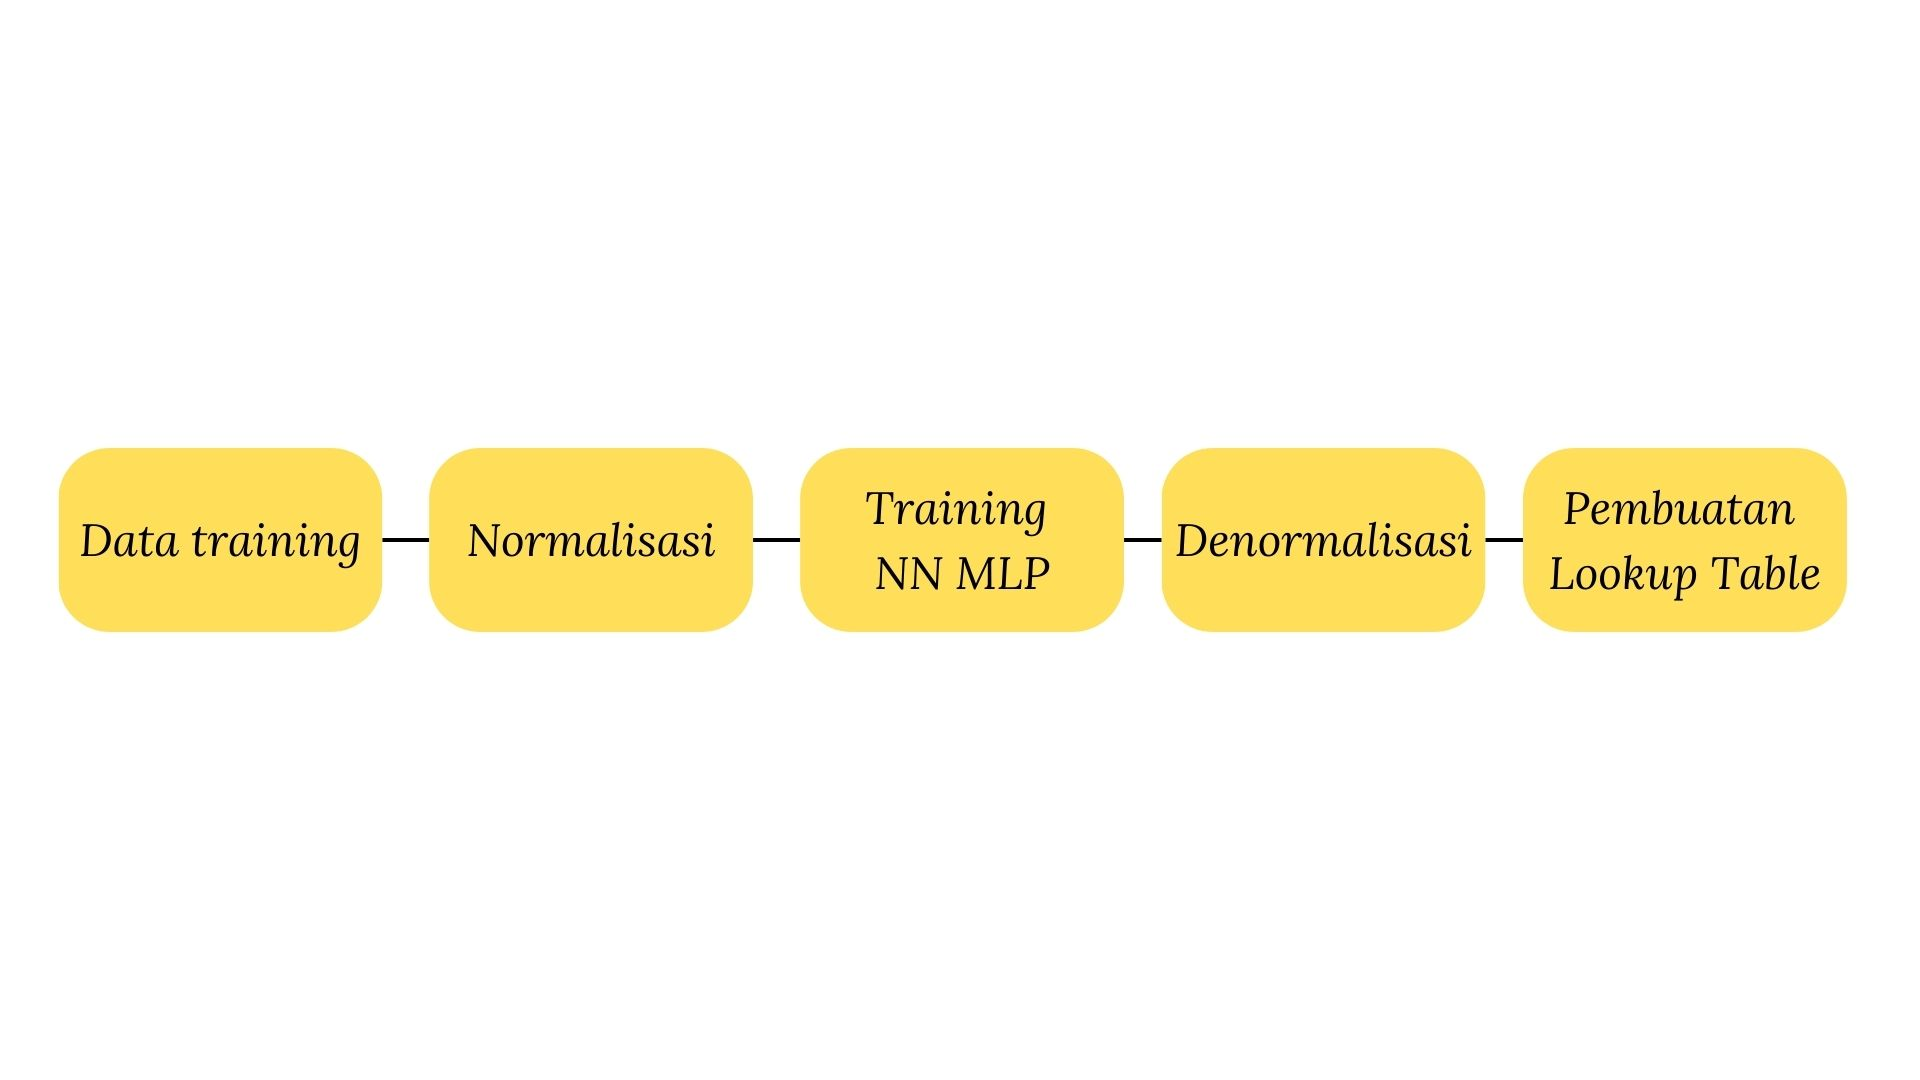
\includegraphics[width=10cm]{gambar/bab3223.jpg}
  \caption{Calibration Process Block Diagram.}
  \label{fig:diag32}
\end{figure}

After all the training data is obtained, the data will be normalized first. The purpose of normalization is to make the data used in the learning process have the same range. In addition, to be able to utilize the activation function used. Here is the normalization formula used:

\begin{equation}
  \begin{aligned}
    normalized\_direction &= \frac{direction\_raw\_value}{180} - 1 \\
  \end{aligned}
\end{equation}

\begin{equation}
  \begin{aligned}
    normalized\_camera\_distance &= \frac{camera\_distance\_raw\_value}{160} - 1 \\
  \end{aligned}
\end{equation}

\begin{equation}
  \begin{aligned}
    normalized\_world\_distance &= \frac{world\_distance\_raw\_value}{600} - 1 \\
  \end{aligned}
\end{equation}

% Dengan menggunakan rumus normalisasi yang telah disebutkan, maka bisa didapat data baru sebagai berikut: 

Using the normalization formula mentioned above, the new data can be obtained as follows: 

\begin{table}[H]
  \caption{Normalized Data Training.}
  \begin{center}
  \begin{tabular}{|c|c|c|c|c|c|}
    \hline
    \rowcolor[HTML]{C0C0C0}
    \textbf{A} & \textbf{B} & \textbf{C} & \textbf{D} & \textbf{E} & \textbf{F} \\
    \hline
    0 deg            & 81 px                & 60 cm            & -1 & -0.49 & -0.90 \\
    0 deg            & 105 px                & 110 cm            & -1 & -0.34 & -0.82 \\
    0 deg           & 143.36 px                & 160 cm            & -1 & -0.10 & -0.73 \\
    10 deg           & 81 px                & 60 cm           & -0.94 & -0.49 & -0.90 \\
    10 deg           & 104.74 px                & 110 cm           & -0.94 & -0.35 & -0.82 \\
    10 deg           & 149.68 px                & 160 cm           & -0.94 & -0.06 & -0.73 \\
    10 deg           & 171.88 px                & 260 cm           & -0.94 & 0.07 & -0.57 \\
    20 deg           & 81.2 px                & 60 cm           & -0.89 & -0.49 & -0.90 \\
    20 deg           & 127.34 px                & 110 cm           & -0.89 & -0.20 & -0.82 \\
    20 deg           & 149.38 px                & 160 cm           & -0.89 & -0.07 & -0.73 \\
    20 deg           & 162.03 px                & 210 cm           & -0.89 & 0.01 & -0.65 \\
    20 deg           & 173.40 px                & 260 cm           & -0.89 & 0.08 & -0.57 \\
    ...           & ...                & ...           & ... & ... & ... \\
    350 deg           & 81.39 px                & 60 cm           & 0.94 & -0.49 & -0.90 \\
    350 deg           & 105.72 px                & 110 cm           & 0.94 & -0.34 & -0.82 \\
    350 deg           & 147.68 px                & 160 cm           & 0.94 & -0.08 & -0.73 \\
    350 deg           & 159.80 px                & 210 cm           & 0.94 & -0.00 & -0.65 \\
    350 deg           & 169.58 px                & 260 cm           & 0.94 & 0.06 & -0.57 \\
    \hline
  \end{tabular}
  \label{tab2}
  \end{center}
\end{table}

With $A$ stand for Direction on Camera, $B$ stand for Distance on Camera, $C$ stand for Distance in the World, $D$ stand for Normalized Direction on Camera, $E$ stand for Normalized Distance on Camera, and $F$ stand for Normalized Distance in the World.

After the normalized data is obtained, the data will be processed using the Multi-Layer Perceptron method. The architecture of the Multi-Layer Perceptron is as follows:

\begin{figure}[H]
  \centering
  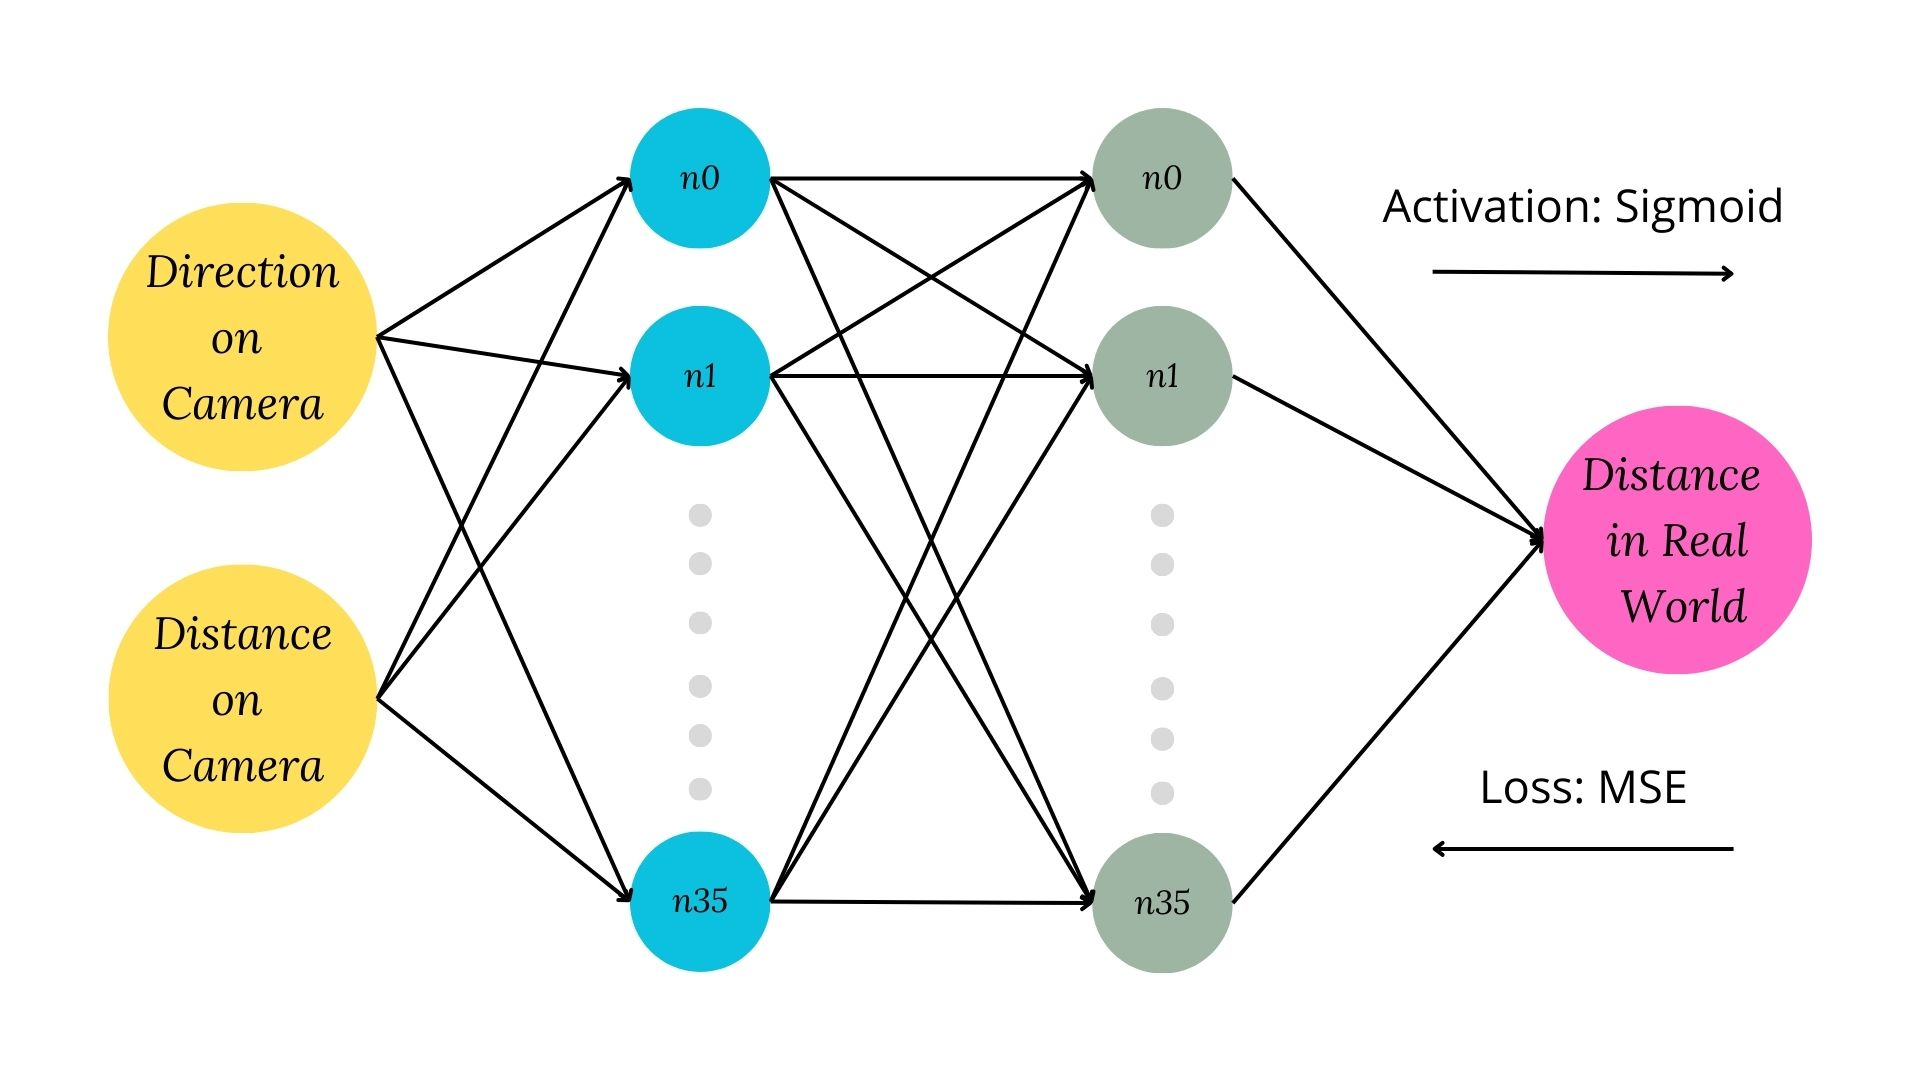
\includegraphics[width=8cm]{gambar/anu.jpg}
  \caption{NN MLP Architecture.}
  \label{fig:diag322}
\end{figure}

The architecture of the Multi-Layer Perceptron consists of 2 hidden layers, each with 36 neurons. Meanwhile, for the input layer consists of 2 neurons in the form of $jarak\_objek\_pada\_kamera$ and $arah\_objek\_pada\_kamera$. The output layer consists of 1 neuron in the form of $jarak\_objek\_pada\_dunia$. The activation function used is Sigmoid. The use of Sigmoid will make the training results more varied and more non-linear.

\begin{equation}
  \begin{aligned}
    f(x) &= \frac{1}{1 + e^{-x}}
  \end{aligned}
\end{equation}

The training process is carried out using the architecture according to the image above. The training process is carried out for 300000 epochs. After the training process is complete, a model will be obtained whose input is the distance and direction on the camera with the output in the form of distance in the real world.

To get the distance and direction data according to the training data in table 1, the data must be denormalized first. Here is the denormalization formula used:

\begin{equation}
  \begin{aligned}
    real\_world\_r &= normalized\_real\_world\_r \times 600 + 600 \\
  \end{aligned}
\end{equation} 

Using the formula above, the actual distance data in the real world can be obtained. The data will be made into a Lookup Table which will then be used in the next process. The making of the Lookup Table is done with two formulas, namely the formula to determine the size of the Lookup Table and the second is the formula to determine the value of each element of the Lookup Table. Here is the formula to determine the size of the Lookup Table:

\begin{equation}
  \begin{aligned}
    size &= \theta\_max \times r\_max \\
  \end{aligned}
\end{equation}

Here is the formula to determine the value of each element of the Lookup Table: 

\begin{equation}
  \begin{aligned}
    index &= \theta \times r\_max + r
  \end{aligned}
\end{equation}

By using the index, the value of each element of the Lookup Table can be obtained. Then the Lookup Table will be saved into a binary file in the robot operating system.


\section{Robot Implementation}
\label{sec:desaindanimplementasi2}

The implementation design on the robot to test the calibration results is by detecting the ball in the field. Here are the steps taken on the IRIS Robot: 

\begin{figure}[H]
  \centering
  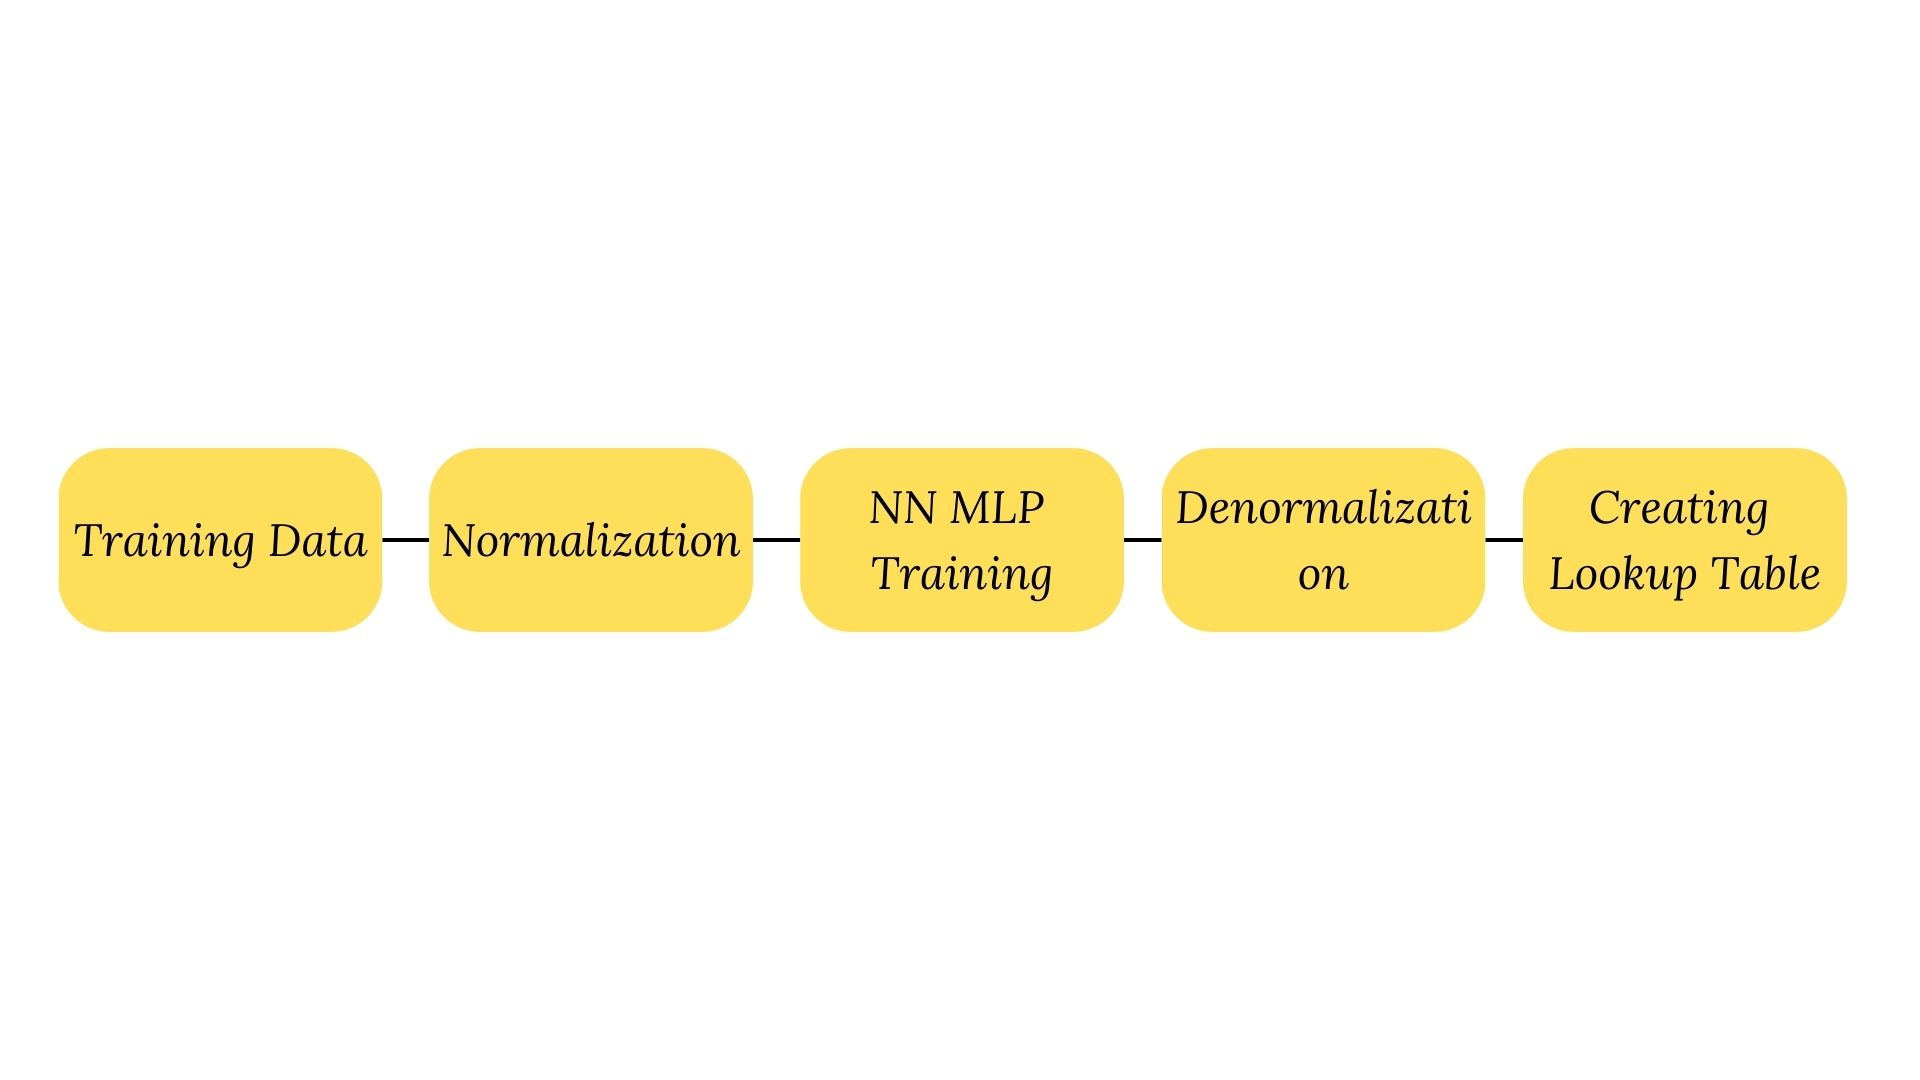
\includegraphics[width=8cm]{gambar/anu3.jpg}
  \caption{Robot Implementation Block Diagram.}
  \label{fig:diag33}
\end{figure}


The camera image on the IRIS Robot is obtained through the Omnivision camera. The image is then processed by a C++ program that has been made by the author. 

The next step after getting the image on the camera is to do color segmentation on the image. Color segmentation is done by comparing the YUV value in the image with the predetermined YUV value. The predetermined YUV value is the YUV value of the ball color. So the output of color segmentation is a binary image. Here is an example of a binary image generated from color segmentation:


\begin{figure}[H]
  \centering
  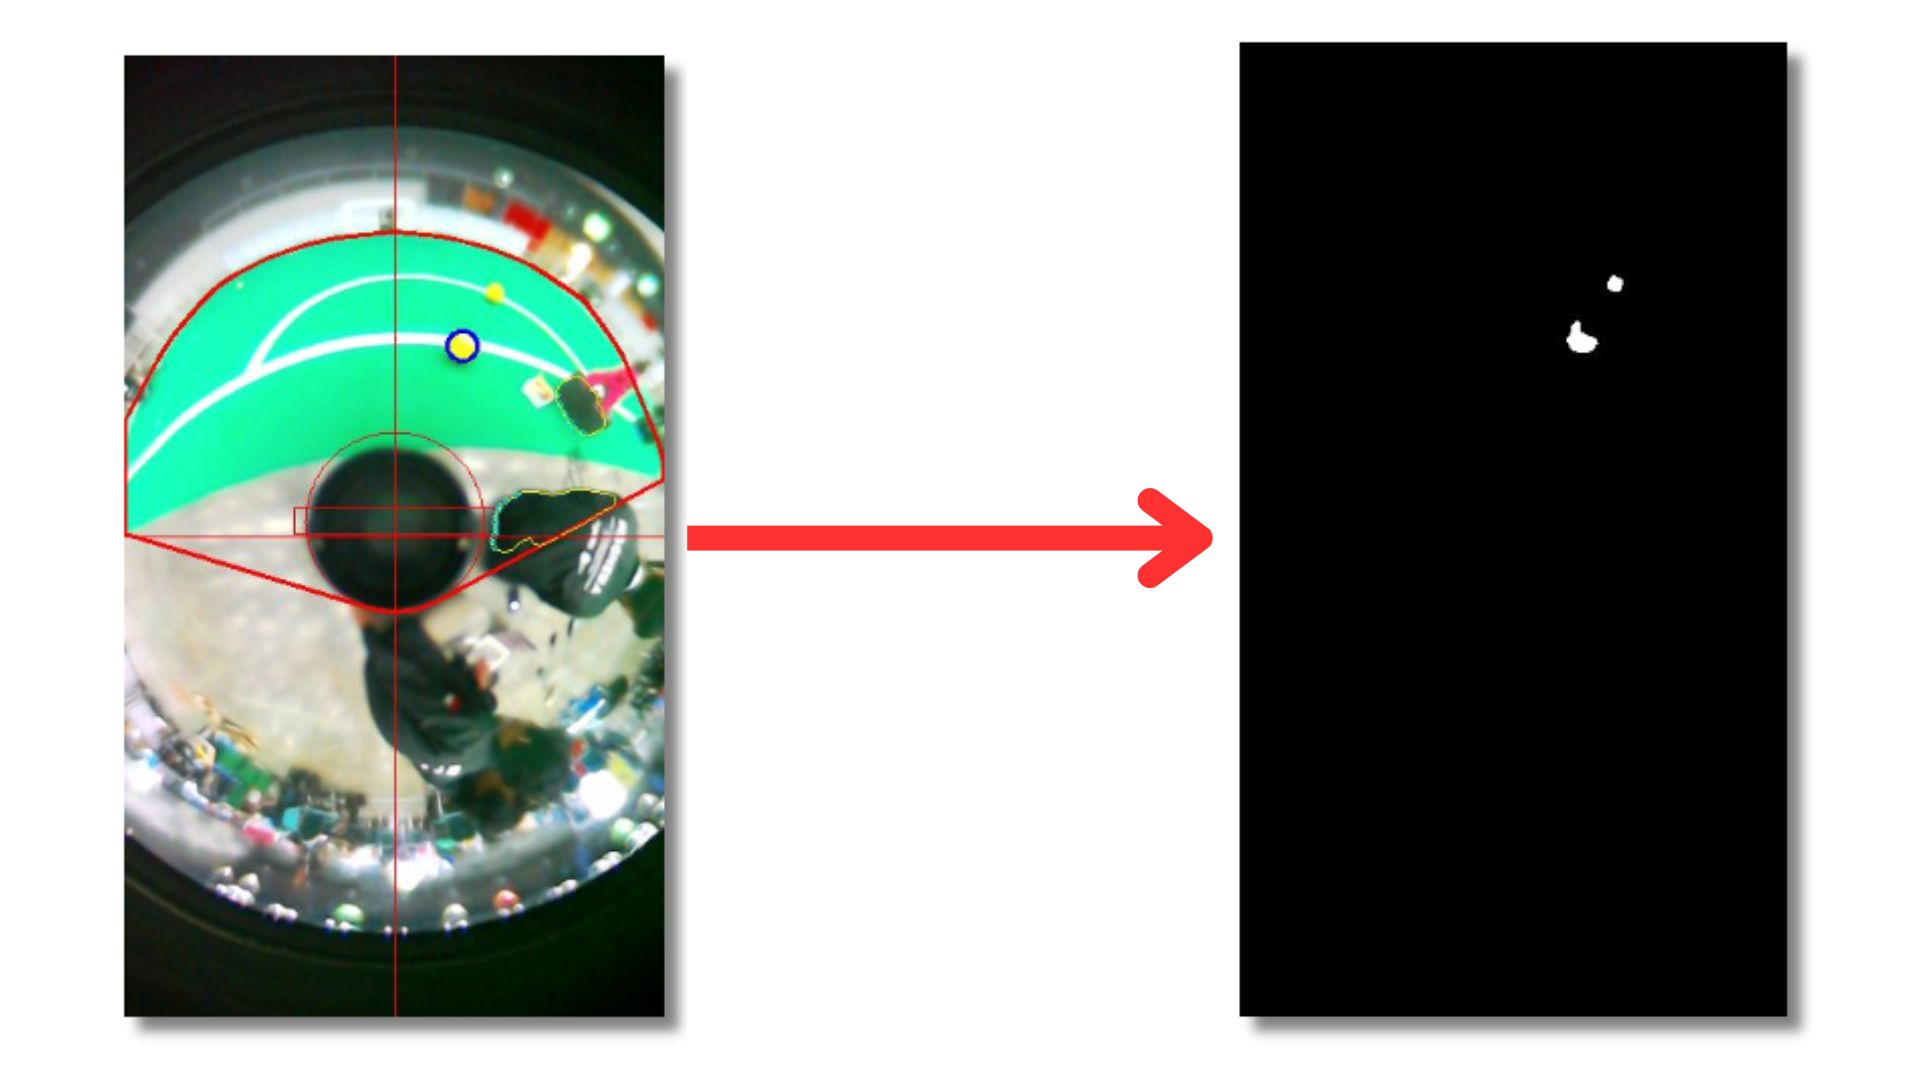
\includegraphics[width=8cm]{gambar/threshold.jpg}
  \caption{Binary and RGB Image.}
  \label{fig:diag332}
\end{figure}

After getting the binary image, the next step is to find the object coordinates in the image. To do this, the following procedure is used: 


\begin{algorithm}[H]
  \caption{Find Ball on Camera}\label{alg:process_lines}
  \begin{algorithmic}[1]
  \Procedure{FindBall}{}
      \For{\text{angle from 0 to 360 with step size 2.5}}
          \State \text{Initialize dist to 0}
          \For{\text{index from 0 to 320}}
              \State $x \gets \text{dist} \times \cos(\text{angle}) + \text{center\_cam\_x}$
              \State $y \gets \text{center\_cam\_y} - \text{dist} \times \sin(\text{angle})$
              \If{\text{ball\_frame\_binary[y][x] == 255}}
                  \State $ball\_x\_on\_kamera \gets x$
                  \State $ball\_y\_on\_kamera \gets y$
                  \State \text{Break}
              \EndIf
              \State $dist \gets \text{dist} + 1$
          \EndFor
      \EndFor
  \EndProcedure
  \end{algorithmic}
\end{algorithm}

\begin{figure}[H]
  \centering
  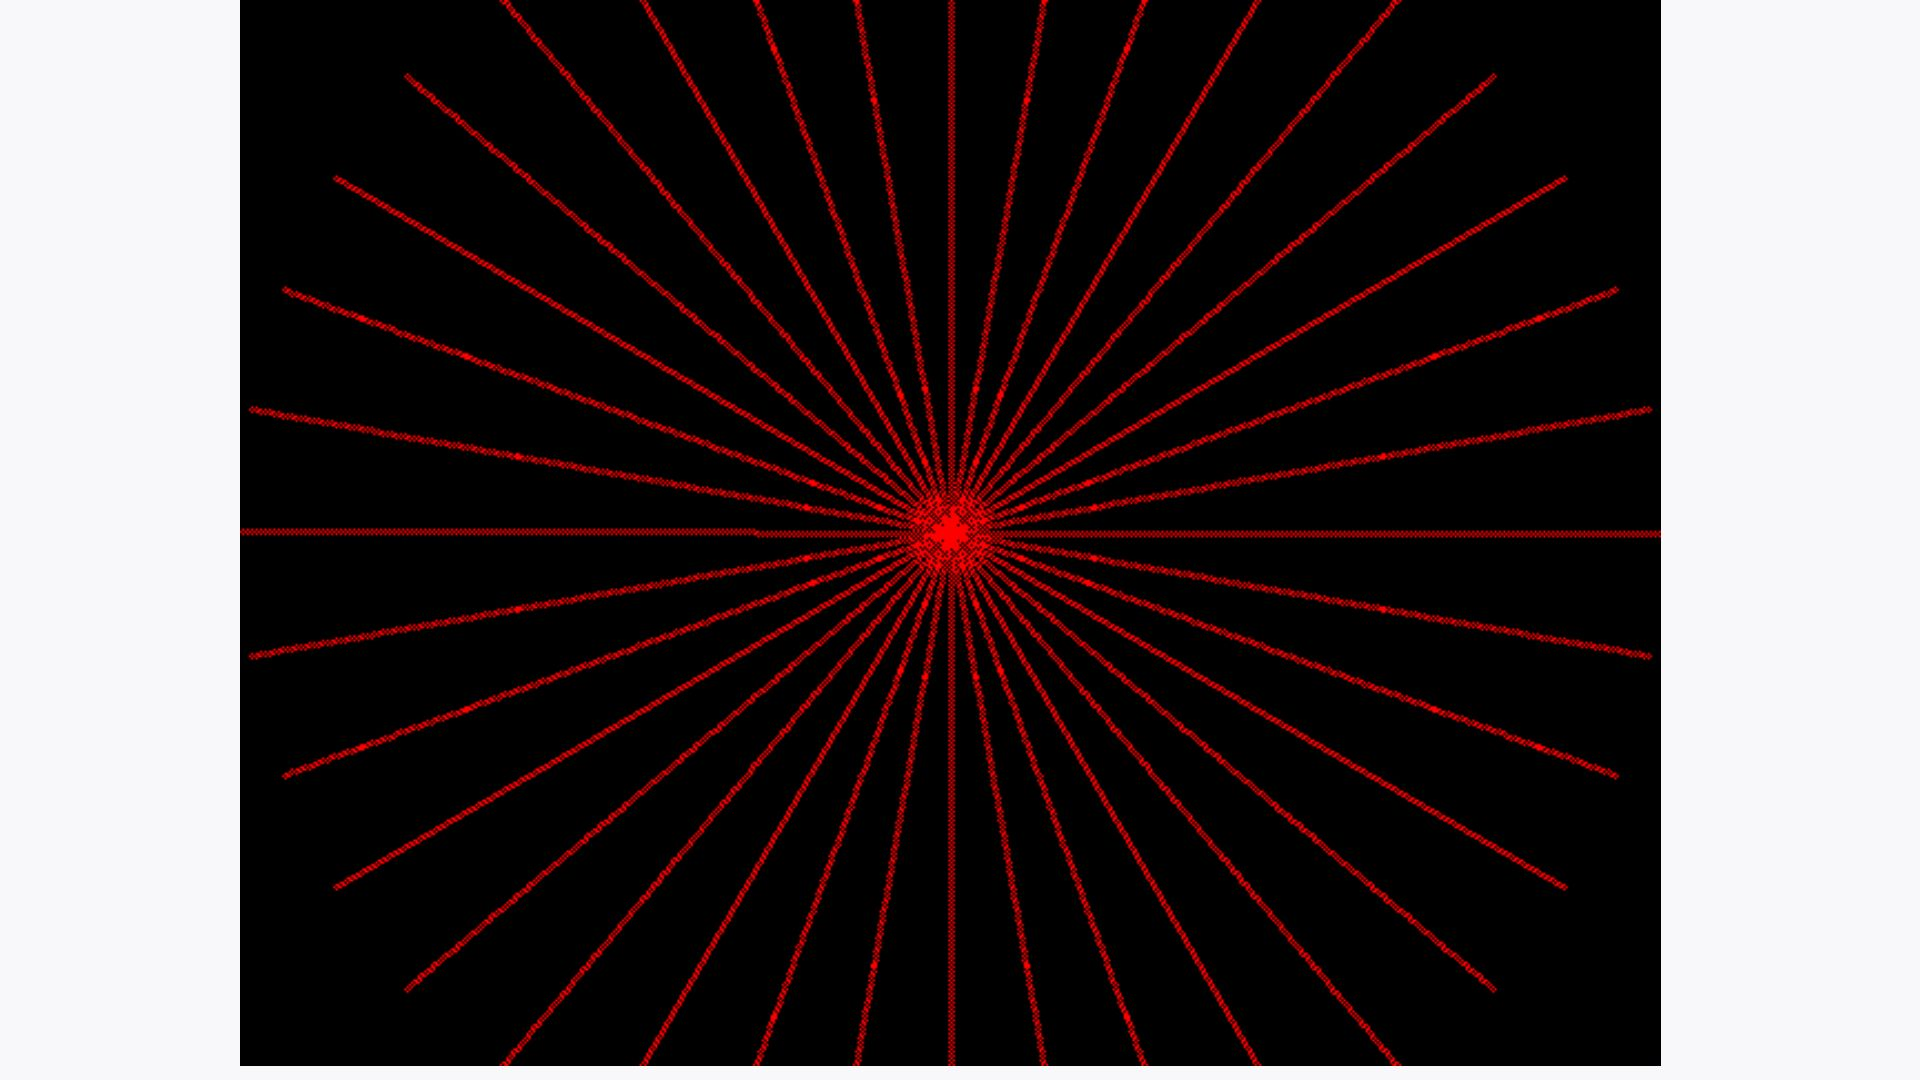
\includegraphics[width=8cm]{gambar/linear.jpg}
  \caption{Linear Scanning Visualization.}
  \label{fig:diag333}
\end{figure}

The meaning of the procedure is to do linear scanning from the center of the camera outwards with an angle of 2.5 degrees. At each angle, a linear scanning will be done from the center of the camera outwards with a distance of 1 pixel. If the pixel at that coordinate has a value of 255, then the coordinate is the ball coordinate on the camera. 

Next, after getting the Cartesian ball coordinates on the camera, the next step is to change the Cartesian coordinates into polar coordinates. Here is the procedure for changing Cartesian coordinates into polar coordinates:

\begin{algorithm}[H]
  \caption{Ball Cartesian Coordinate to Polar Coordinate}\label{alg:prosedur4}
  \begin{algorithmic}[1]
  \Procedure{BallCartesian2Polar}{}
      \State $dx \gets ball\_x\_on\_cam - x\_center\_cam$
      \State $dy \gets y\_center\_cam - ball\_y\_on\_cam$
      \State $ball\_\theta\_cam \gets \arctan(\frac{dy}{dx})$
      \State $ball\_distance\_cam \gets \sqrt{dx^2 + dy^2}$
  \EndProcedure
  \end{algorithmic}
\end{algorithm}

Next, after getting the distance and direction data of the ball on the camera, the distance of the ball in the real world can be obtained by reading the Lookup Table. Here is the procedure for reading the Lookup Table:

\begin{algorithm}[H]
  \caption{Reading Lookup Table}\label{alg:prosedur5}
  \begin{algorithmic}[1]
  \Procedure{ReadLookupTable}{}
      \State $index \gets ball\_\theta\_cam \times r\_max + ball\_distance\_cam$
      \State $ball\_distance\_world\_local \gets lookup\_table[index]$
      \State $ball\_\theta\_world\_local \gets ball\_\theta\_cam$
  \EndProcedure
  \end{algorithmic}
\end{algorithm}


After getting the distance and direction of the ball in the real world, the position of the ball in the real world can be obtained. However, the ball position is still a local ball position, which means that the ball position is still relative to the robot. To get the global ball position, the ball position must be added to the robot's position and orientation. Here is the procedure to get the global ball position:

\begin{algorithm}[H]
  \caption{Local to Global World Model for Ball}\label{alg:prosedur6}
  \begin{algorithmic}[1]
    \Procedure{BallLocal2Global}{}
      \State $ball\_\theta\_global \gets angle\_px + robot\_pose\_\theta - 90$
      \State $ball\_x\_global \gets robot\_pose\_x + ball\_distance\_world\_local \times \cos(\text{DEG2RAD} \times ball\_\theta\_global)$
      \State $ball\_y\_global \gets robot\_pose\_y + ball\_distance\_world\_local \times \sin(\text{DEG2RAD} \times ball\_\theta\_global)$
  \EndProcedure
  \end{algorithmic}
\end{algorithm}

By using the procedure above, the position of the ball in the real world can be obtained in the form of $ball\_x\_global$ and $ball\_y\_global$.

% \section{Calibration Testing Design}
% \label{sec:desaindanimplementasi3}
